\documentclass[a4paper, 12pt]{article}

\usepackage[utf8]{inputenc}
\usepackage[spanish,es-noquoting]{babel}
\usepackage{enumitem}
\usepackage[a4paper,bindingoffset=0.2in,%
            left=1in,right=1in,top=1in,bottom=1in,%
            footskip=.25in]{geometry}
\linespread{1.25}

\usepackage{graphicx}
\usepackage{hyperref}
\usepackage{pdfpages}
\usepackage{pdflscape}



\title{Memoria de seguimiento}
\author{Alejandro García Castellanos\\z17m008}

\tolerance=1
\emergencystretch=\maxdimen
\hyphenpenalty=10000
\hbadness=10000


\begin{document}
\maketitle 

\section{Resumen del trabajo realizado}
Como comenté en las tareas del plan de trabajo comencé repasando los contenidos de la asignatura de Topología Computacional. Una vez terminado, estudié el siguiente articulo: \textit{\href{https://link.springer.com/content/pdf/10.1007/s00454-006-1276-5.pdf}{Cohen-Steiner, David \& Edelsbrunner, Herbert \& Harer, John. (2005). Stability of Persistence Diagrams. Discrete \& Computational Geometry - DCG. 37. 263-271. 10.1007/s00454-006-1276-5}}. Profundizando en las cuestiones y pasos de la demostración que más dificultad me suponían.

Tras comprender el resultado y la demostración del teorema, escribí la sección de conocimientos previos necesarios para hacer autocontenida el trabajo. Para ello he hecho uso de libros, artículos y conferencias para tomar sus explicaciones y definiciones como referencia. Por último he introducido el teorema de estabilidad tanto para la distancia Hausdorff como para la distancia Bottleneck, con el fin de poner en contexto los algoritmos necesarios para la implementación.

Para la sección de implementación, hice una búsqueda de los diversos métodos de calcular las distancias y escribí su funcionamiento explicado en la memoria. Además he estado investigando sobre el funcionamiento de diversas librerías de Python que me pueden ser de utilidad a la hora de implementar los algoritmos propuestos.
\section{Modificaciones al Plan de Trabajo}
\subsection{Revisión de la lista de objetivos del trabajo}
Se ha añadido la implementación de la distancia Hausdorff a los objetivos del trabajo, ya que la demostración propuesta en el articulo previamente mencionado, demuestra primero la estabilidad para esta distancia. Por tanto es conveniente implementarla para ilustrar este resultado.

Luego, la lista de objetivos del trabajo es:
\begin{itemize}
	\item Buscar referencias que contengan el enunciado y la demostración del Teorema de estabilidad.
	\item Estudiar y entender estas referencias.
	\item Implementar el cálculo de las distancias de Bottleneck y Hausdorff entre diagramas de persistencia.
	\item Ilustrar el Teorema de estabilidad sobre distintos conjuntos de datos.
	\item Redactar la memoria y preparar la presentación
\end{itemize}

\subsection{Revisión de la lista de tareas}
La lista de tareas se ve modifica en dos puntos. El primero en el hecho de añadir la implementación de la distancia Hausdorff y el segundo en la redacción de los algoritmos para el cálculo de las distancias, la cual no se había considerado en el Plan de Trabajo original.

Es por ello que la lista tareas para la realización del trabajo es:
\begin{itemize}
	\item \textbf{Preparación}
	\begin{itemize}
		\item Buscar referencias que contengan el enunciado y la demostración del Teorema de estabilidad.
		\item Repasar los contenidos de la asignatura de Topología Computacional.
	\end{itemize}
	
	\item \textbf{Realización de los objetivos principales}
	\begin{itemize}
		\item Estudiar y entender estas referencias.
		\item Implementar el cálculo de las distancias Bottleneck y Hausdorff entre diagramas de persistencia
		\begin{enumerate}
			\item Búsqueda de los algoritmos.
			\item Implementación sobre clase de complejos simpliciales programada en la asignatura de Topología Computacional.
			\item Testing de las nuevas funcionalidades.
		\end{enumerate}
	\end{itemize}
	
	\item \textbf{Elaboración de la Memoria y Presentación}
	\begin{itemize}
		\item \textbf{Memoria}
		\begin{itemize}
			\item Redactar conocimientos previos requeridos para la comprensión del teorema.
			\item Redactar Teorema de estabilidad y su demostración.
			\item Redactar algoritmos para el cálculo de las distancias.
			\item Ilustrar el teorema a través de su implementación.
		\end{itemize}
		\item Elaboración y preparación de la presentación.
	\end{itemize}
	
\end{itemize}

\section{Revisión del Diagrama de Gantt}
Debido a un error de estimación del tiempo requerido para la realización de la parte de ``Conocimientos previos'', se ve desplazada la planificación de las tareas: ``Redactar Teorema y demostración'', ``Implementar distancias'' e ``Ilustrar conocimientos''. Y se ha incorporado en el Diagrama de Gantt la tarea ``Redactar algoritmos''.

Además, no se tuvo en consideración el tiempo de estudio de los algoritmos de las distancias en la planificación de la tarea ``Estudiar y entender las referencias''.

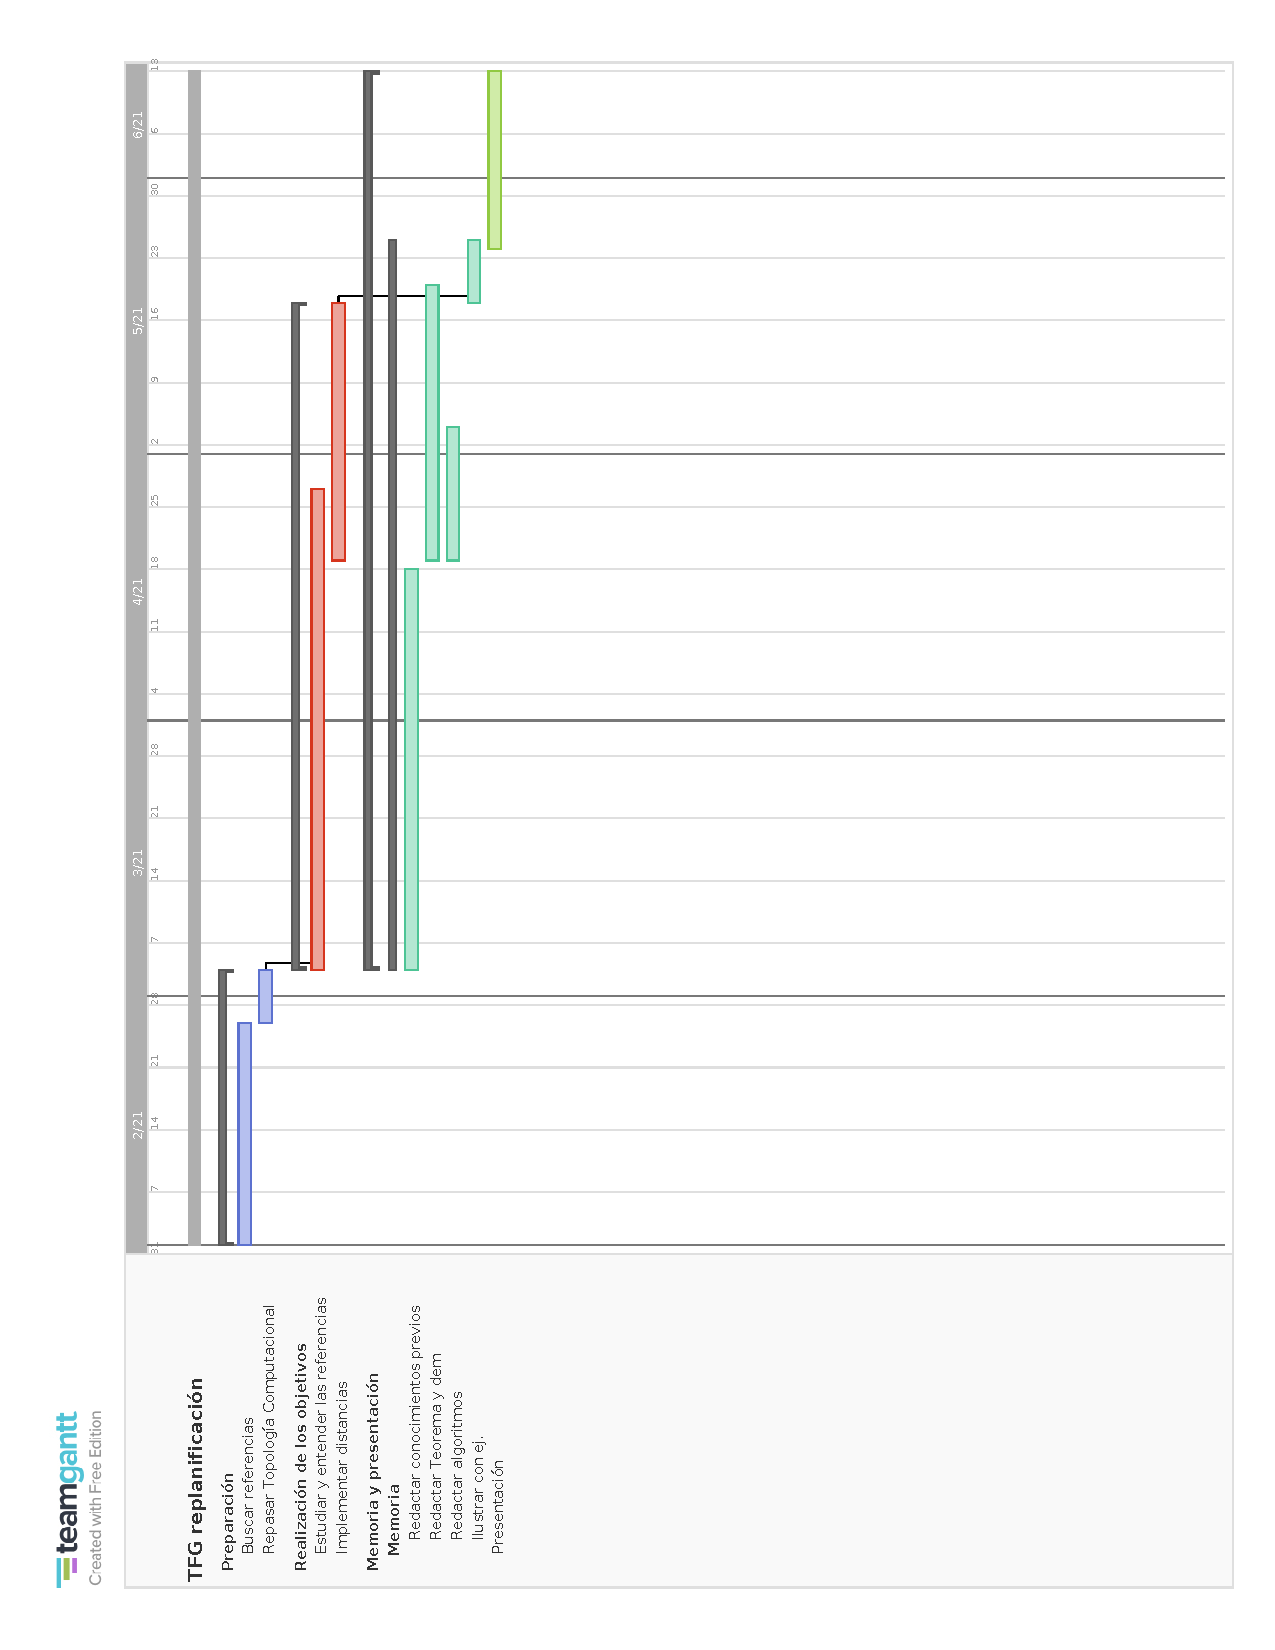
\includepdf{TFG_gantt}

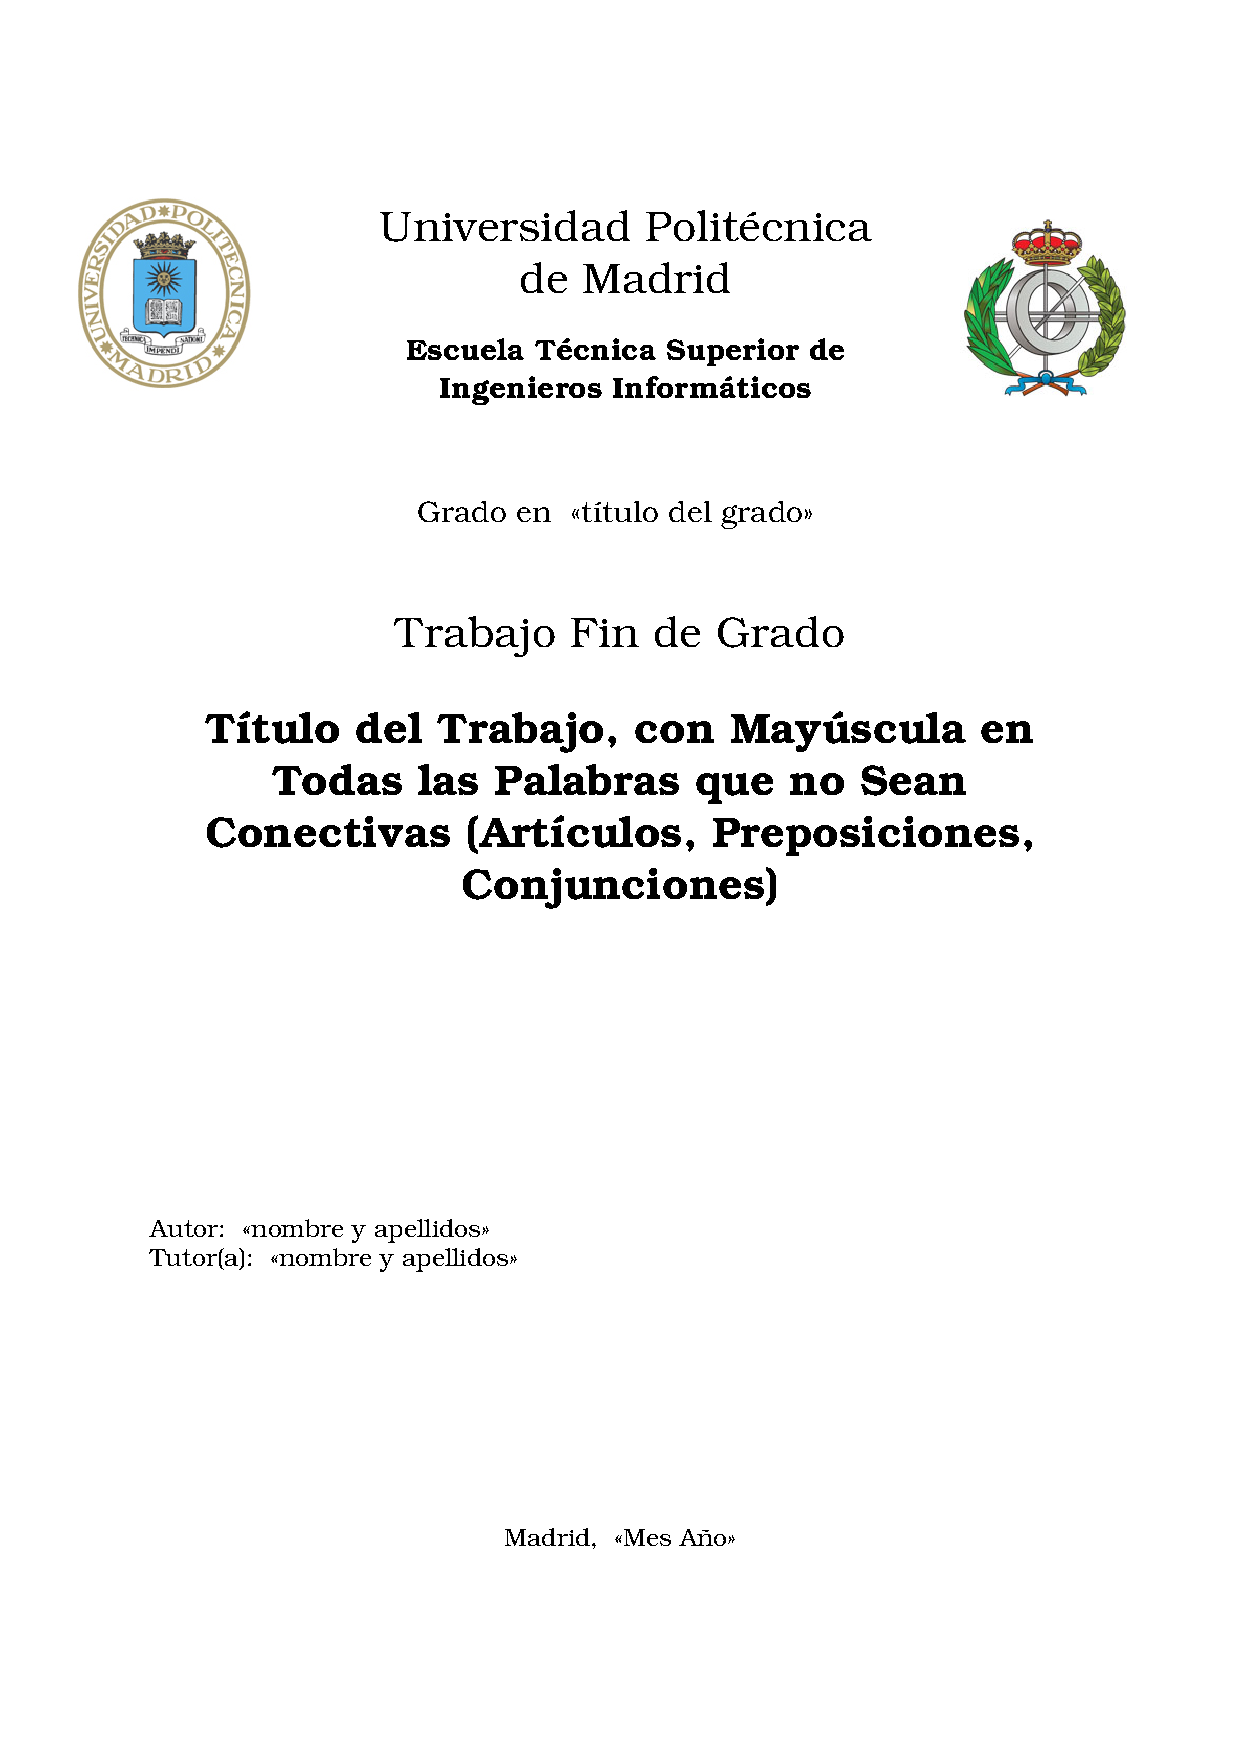
\includepdf[pages=-]{../tfg_latex/TFG_Teorema_Estabilidad}


\end{document}





